\documentclass[a4paper, 12pt]{book}
% preamble.tex

\usepackage[utf8]{inputenc}
\usepackage[T1]{fontenc}
\usepackage[english]{babel} % Ho cambiato in italian, supponendo che la maggior parte del testo sia in italiano
\usepackage{amsmath}
\usepackage{amssymb}
\usepackage{graphicx}
\usepackage{hyperref}
\usepackage{geometry}
\usepackage{fontspec} % Utile per Xetex/LuaLaTeX ma mantenuto
\usepackage{booktabs}
\usepackage{amsthm}
\usepackage{enumitem}
\usepackage{caption}
\usepackage{thmtools}
\usepackage{standalone} % Già presente nel tuo elenco
\usepackage{tkz-euclide}
\usepackage{graphicx}
\usepackage[T1]{fontenc}
\usepackage{wesa}

% --- PACCHETTI AGGIUNTI PER LA FORMATTAZIONE ---
\usepackage{parskip}  % Aggiunge spazio tra i paragrafi (stile "blocco")
\usepackage{fancyhdr} % Per intestazioni e piè di pagina personalizzati

% --- IMPOSTAZIONI GEOMETRIA E FONT ---
\geometry{a4paper, margin=1in}

% Configura lo stile 'plain' (usato da \maketitle e \tableofcontents)
% per essere coerente con il piè di pagina
\fancypagestyle{plain}{
    \fancyhf{} % Pulisce
    \cfoot{\thepage} % Mette solo il numero di pagina
    \renewcommand{\headrulewidth}{0pt} % Niente linea su queste pagine
}

% Configurazione Header/Footer per le altre pagine
\pagestyle{fancy}
\fancyhead{} % Pulisce l'intestazione
\fancyfoot{} % Pulisce il piè di pagina
\fancyhead[L]{\nouppercase{\rightmark}} % Nome Sezione a sinistra (o Chapter)
\fancyhead[R]{\nouppercase{\leftmark}}  % Nome Capitolo a destra (o Sezione)
\fancyfoot[C]{\thepage} % Numero di pagina al centro
\renewcommand{\headrulewidth}{0.4pt}
\renewcommand{\footrulewidth}{0pt}


% --- DEFINIZIONI TEOREMI ---
% (Questa parte è cruciale per la tua struttura)
\newtheoremstyle{mythmstyle}%
    {}%
    {}%
    {\itshape}%
    {}%
    {\bfseries}%
    {}%
    { }%
    {\thmname{#1}\thmnumber{ #2}%
    \thmnote{: #3\addcontentsline{toc}{subsubsection}{{\itshape#1}: #3}}. }

% 2. Imposta questo stile come quello ATTUALE
\theoremstyle{mythmstyle}

\newtheorem{theorem}{Th}[section]
\newtheorem{definition}{Def}[section]
\newtheorem{proposition}{Prop}[section]
\newtheorem{corollary}{Cor}[section]
\newtheorem{algorithm}{Alg}[section]
\newtheorem{lemma}{Lemma}[section]
\newtheorem*{remark}{Rem}

% Definizioni utili per il Main file
\newcommand{\inputlesson}[1]{\clearpage\input{#1}\clearpage} % Comando per input lezione
\usepackage[x11names]{xcolor}
\usepackage{tikz}
\usetikzlibrary{shapes,fit}
\usepackage{amsmath} % Required for align environment


\begin{document}
\setcounter{chapter}{2}
\chapter[ ]{Week 13-19 October}
\section{Spectral efficiency for finite-length codewords}

We can reach the Shannon bound only by pushing $N$ to infinity; only if we're sending a \textit{really} long codeword can we reach the capacity. We'd need to wait a long time (an \textit{infinite} amount of time, I think) to fill that codeword and then we'd have to wait lots of latency in order to receive such a large signal.

We can show that by using small (non infinite!) $N$ values, we don't reach the capacity and we can indeed show to which spectral efficiency we actually get!

\begin{equation}
\frac{R}{B} = C - \sqrt{\frac{V}{N}} Q^{-1}(p_e) + \mathcal{O}\left(\frac{\log N}{N}\right) \text{.} \tag{1.143}
\end{equation}

\textit{How below} we stay depends on $N, V, p_e$; we don't need to remember the capacity, but we do need to remember the fact that \textbf{it's lower when compared to the capacity}.

Takeaway points are:
\begin{enumerate}[label=\textcolor{gray}{\arabic*.}]
    \item If the \textbf{block length} $N$ \textbf{increases}, we get closer to the \textbf{ideal} capacity
    \item If the \textbf{probability of error decreases}, we get closer to the \textbf{ideal} capacity (since $p_e \downarrow \implies Q \uparrow \implies (1/Q) \downarrow$)
    \item If the \textbf{information density has a lower variance} (totally intuitively, i.e. if input/output are more related), we get closer to the \textbf{ideal} capacity
\end{enumerate}

$V$ is the variance of the information density, defined as
\begin{equation}
V = \text{var}[i(s;y)] \text{.} \tag{1.144}
\end{equation}

This is a really cool result, as it allows us to understand how far away we are from ideal capacity.

% Riquadro Rosso
\begin{tcolorbox}[colframe=red!80!white, colback=white, boxrule=1pt, arc=2pt]
    \textcolor{red}{\textbf{About the exam}}

    The sections published on the website are the program for the exam.
\end{tcolorbox}

\section{MMSE estimation}

\noindent
\textcolor{green!60!black}{Ref: \hfill Chapter\_1\_EE\_381S\_Spg\_2019,}\\
\textcolor{green!60!black}{08.1\_pp\_3\_56\_A\_primer\_on\_information\_theory\_and\_MMSE\_estimation, page 37.}

% Riquadro Verde (Note logistiche)
\begin{tcolorbox}[sharp corners, boxrule=0pt, leftrule=2pt, colframe=green!60!black, colback=green!5, left=5pt, top=3pt, bottom=3pt]
    Probably next week we'll receive an email about the 1st of November and about where the lesson has been moved.
    
    18th, 19th of 20th of November (and even more), professor will be in Paris. We'll have 3 extra dates, probably wed 16:30-18:30. We'll be able to find all the information about this on elearning.
\end{tcolorbox}

\subsection{Intro to MMSE estimation, scalar estimator (and the properties an estimator should have)}

Today we'll do Minimum Mean Squared Error Estimation: MMSE estimation.
This is something between telecommunications and control engineering.
It goes back to Gauss and friends, but we've had much progress in the 20th century after the world war; the two major achievements are the Wieman and Calman filter.
Without the Calman filter, we wouldn't have gone to the moon.

We'll go over different MMSE estimators; usually \textbf{estimating means we want to estimate a parameter}; here we have a transmitter and at the receiver we want to estimate the transmitted signal. This is the idea of this.
This is not the only estimator though (we've seen MAP, ML, MD, \ldots).
The last part of the chapter shows that the mutual information can be derived, instead of the usual way we've seen till now, as a derivate of what we'll call information MSE.

Our problem is to estimate a signal in noise
\begin{align*}
y = \sqrt{\rho}s + z \;;
\end{align*}
we have the observation $y$, we have $\sqrt{\rho}$, where $\rho$ is the SNR and then we'll have $z$, Gaussian noise and $s$, unknown.
We have some statistical information, such as:
\begin{itemize}
    \item Posterior probability, probability density of s given y, $f_{s|y}(\cdot)$
    \item We have the likelihood function: we know the probability density of y given s, $f_{y|s}(\cdot)$
    \item Sometimes we have even the probability density of $s$, $f_s(\cdot)$!
\end{itemize}

% Riquadro Blu Unificato (Pagina 1 + Pagina 2)
\begin{tcolorbox}[colframe=cyan!80!blue, colback=white, boxrule=1pt, arc=2pt]
    \textcolor{cyan!80!blue}{\textbf{Estimation problem, solution $\hat{s}(y)$}}

    We want to find the solution $\hat{s}(y)$ which minimizes the MSE, $\mathbb{E}[\|s - \hat{s}(y)\|^2]$.
    
    \vspace{0.5em}
    \hrule
    \vspace{0.5em}
    
    We can see this as a statement, but we'll do exercise 1.34 about this; the solution is
    \begin{align}
    \hat{s}(y) = \mathbb{E}[s|y] \;. \tag{1.151}
    \end{align}
\end{tcolorbox}

\vspace{1em}

When we make an estimator, we first of all need to check that the estimator is \textbf{unbiased}, aka that on average it gives me the actual quantity that I want to estimate: "If I estimate many times, I should get my estimate!".

The thermometer is kind of estimating the temperature; the thermometer might be biased, though. The termometer might give always 1 degree more than the temperature.
A good estimator should on average give a temperature of 24 if the temperature actually is 24.

This is \textbf{unbiased} in the sense that
\begin{align}
\mathbb{E}[\hat{s}(y)] = \mathbb{E}[\mathbb{E}[s|y]] \stackrel{*}{=} \mathbb{E}[s] \;. \tag{1.153}
\end{align}

% Riquadro Verde (Nota teorema)
\begin{tcolorbox}[sharp corners, boxrule=0pt, leftrule=2pt, colframe=green!60!black, colback=green!5, left=5pt, top=3pt, bottom=3pt]
    $*$ comes from the \textcolor{green!60!black}{theorem of total expectation}, which, by definition is such that
    \begin{align*}
    \underset{y}{\mathbb{E}}[\underset{s}{\mathbb{E}}[s|y]] = \underset{s}{\mathbb{E}}[s] \;.
    \end{align*}
\end{tcolorbox}

The estimator \textbf{must satisfy orthogonality}; if we multiply the error by \textbf{any function} of the observation, it must be equal to 0:
\begin{align*}
\mathbb{E}[g(y^*) (s - \hat{s}(y))] = 0 \quad \forall \text{ function } g(\cdot) \;.
\end{align*}

% Riquadro Verde (Nota coniugato)
\begin{tcolorbox}[sharp corners, boxrule=0pt, leftrule=2pt, colframe=green!60!black, colback=green!5, left=5pt, top=3pt, bottom=3pt]
    We're conjugating $y$; at the same time, $g$ can contain a conjugate, so it's whatever: the conjugate is irrelevant.
    The conjugate will be useful when we'll manipulate the problem later.
\end{tcolorbox}

Let's give an euristic interpretation of orthogonality: if we have a plane with two vectors ($y, z$, at least I think) and a vector going out of the plane ($s$); we want to give the best estimation of the vector which is going out of the plane:

\begin{figure}[h!]
    \centering
    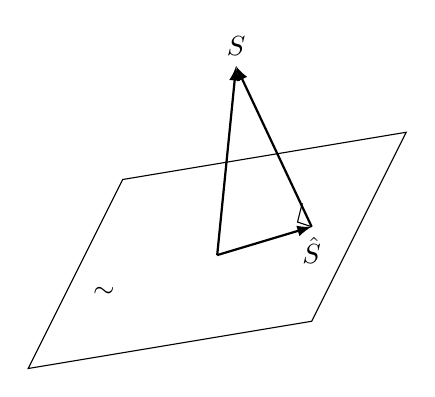
\begin{tikzpicture}[scale=1.2, >=latex]
        % Piano (parallelogramma)
        \draw (0,0) -- (3,0.5) -- (4,2.5) -- (1,2) -- cycle;
        
        % Scarabocchio 'm' sul piano
        \node at (0.8, 0.8) {$\sim$}; 
        
        % Coordinate Origine (approssimata sul piano)
        \coordinate (O) at (2, 1.2);
        
        % Vettore s (uscente dal piano)
        \coordinate (S) at (2.2, 3.2);
        \draw[->, thick] (O) -- (S) node[above] {$S$};
        
        % Vettore s_hat (proiezione sul piano)
        \coordinate (S_hat) at (3, 1.5);
        \draw[->, thick] (O) -- (S_hat) node[below] {$\hat{S}$};
        
        % Vettore errore (ortogonale)
        \draw[->, thick] (S_hat) -- (S);
        
        % Simbolo angolo retto
        \draw (S_hat) -- ++(-0.15, 0.05) -- ++(0.05, 0.2); 

    \end{tikzpicture}
    \caption{Interpretazione geometrica dell'ortogonalità: l'errore di stima è ortogonale al piano delle osservazioni.}
\end{figure}

We'll estimate the vector which is out of the plane, we'll have that our estimate is the projection of the vector on the plane and the error will be orthogonal to the plane (as can be seen in the figure).

We'll also have that the error is also orthogonal to $\hat{s}$ and to what it's available.

And what actually is the MMSE (until now we've only seen the estimator!)? It's the actual error we're making:
\begin{equation}
\text{MMSE}(\rho) = \mathbb{E}[\|s - \mathbb{E}[s|y]\|^2] \text{.} \tag{1.156}
\end{equation}
In this equation it's important to look at the fact that the MMSE is only dependent on $\rho$.

\subsection{MMSE estimator for a Complex Gaussian scalar through a channel}

Let's say we have $y = \sqrt{\rho}s + z$ with
$$
z \sim \mathcal{N}_{\mathbb{C}}(0,1) \implies y|s \sim \mathcal{N}_{\mathbb{C}}(\sqrt{\rho}s, 1) \implies f_{y|s} = \frac{1}{\pi} e^{-|y-\sqrt{\rho}s|^2}
$$

% Riquadro verde
\begin{tcolorbox}[sharp corners, boxrule=0pt, leftrule=2pt, colframe=green!60!black, colback=green!5, left=5pt, top=3pt, bottom=3pt]
    We fix $s$; we can try and see what $y|s$ is: it's a complex Gaussian with mean $\sqrt{\rho}s$ and variance 1.
\end{tcolorbox}

Let's look at the solution:
\begin{align*}
\hat{s}(y) &= \mathbb{E}[s | y=y] \\
&= \int s f_{s|y}(s|y) \, \mathrm{d}s \\
&= \int \frac{s f_{y|s}(y|s) f_s(s)}{\int f_{y|s}(y|s) f_s(s) \, \mathrm{d}s} \, \mathrm{d}s \\
&= \frac{\int s f_{y|s}(y|s) f_s(s) \, \mathrm{d}s}{\int f_{y|s}(y|s) f_s(s) \, \mathrm{d}s} \\
&= \frac{\int s e^{-|y-\sqrt{\rho}s|^2} f_s(s) \, \mathrm{d}s}{\int e^{-|y-\sqrt{\rho}s|^2} f_s(s) \, \mathrm{d}s}
\end{align*}

% Riquadro verde in basso
\begin{tcolorbox}[sharp corners, boxrule=0pt, leftrule=2pt, colframe=green!60!black, colback=green!5, left=5pt, top=3pt, bottom=3pt]
    We go from $f_{s|y}$ to $f_{y|s}$ by using the Bayes theorem.
    
    We can also have $f_y$ as
    $$
    f_y(Y) = \int f_{y,s}(Y, S) \, \mathrm{d}S = \int f_{y|s}(Y|S) f_s(S) \, \mathrm{d}S \;,
    $$
    from the marginalization rules.
\end{tcolorbox}


Then specifically, for Gaussian signals,
\begin{align}
\hat{s}(y) &= \frac{\int s e^{-|y-\sqrt{\rho}s|^2} e^{-|s|^2} \, \mathrm{d}s}{\int e^{-|y-\sqrt{\rho}s|^2} e^{-|s|^2} \, \mathrm{d}s} \tag{1.167} \\
&= \frac{\int s e^{-|\frac{|y|^2}{1+\rho} - \sqrt{1+\rho}s - \frac{\sqrt{\rho}}{1+\rho}y|^2} \, \mathrm{d}s}{\int e^{-|\frac{|y|^2}{1+\rho} - \sqrt{1+\rho}s - \frac{\sqrt{\rho}}{1+\rho}y|^2} \, \mathrm{d}s} \tag{1.168} \\
&= \frac{\int s e^{-|s - \frac{\sqrt{\rho}}{1+\rho}y|^2 / \frac{1}{1+\rho}} \, \mathrm{d}s}{\int e^{-|s - \frac{\sqrt{\rho}}{1+\rho}y|^2 / \frac{1}{1+\rho}} \, \mathrm{d}s} \tag{1.169}
\end{align}

which can be notices to be the mean over the PDF of a complex gaussian distribution of
$$
s' \sim \mathcal{N}_{\mathbb{C}} \left( \frac{\sqrt{\rho}}{1+\rho}y, \frac{1}{1+\rho} \right) \;,
$$
and we can then rewrite the values in (1.169) as
$$
= \frac{\mathbb{E}[s']}{1} = \frac{\sqrt{\rho}}{1+\rho}y \;.
$$

% Riquadro Viola (Passaggi algebrici)
\begin{tcolorbox}[colframe=violet!80!white, colback=white, boxrule=1pt, arc=2pt]
    \textcolor{violet}{\textbf{About the passages from (1.167)}}

    To simplify the exponent in both numerator and denominator:
    $$
    -|y - \sqrt{\rho}s|^2 - |s|^2
    $$
    We expand:
    $$
    |y - \sqrt{\rho}s|^2 = |y|^2 - 2\Re(y^*\sqrt{\rho}s) + \rho|s|^2
    $$
    So,
    $$
    -|y - \sqrt{\rho}s|^2 - |s|^2 = -|y|^2 + 2\Re(y^*\sqrt{\rho}s) - (1+\rho)|s|^2 \;.
    $$
    Our aim now is to try and isolate $s$ from $y$; we then consider that for $a, b \in \mathbb{R}$,
    $$
    |as + by|^2 = a^2|s|^2 + 2ab\Re(y^*s) + b^2|y|^2 \;;
    $$
    if we look at the previous expression (forgetting for now of the sign flip), we can impose
    $$
    a = \sqrt{1+\rho} \;,
    $$
    from which follows that
    $$
    ab = -\sqrt{\rho} \implies b = - \frac{\sqrt{\rho}}{\sqrt{1+\rho}} \;,
    $$
    giving that
    $$
    -|y - \sqrt{\rho}s|^2 - |s|^2 = -a^2|s|^2 + 2ab\Re(y^*s) - |y|^2 :
    $$
\end{tcolorbox}
% --- Continuazione del riquadro viola della pagina precedente ---
\begin{tcolorbox}[colframe=violet!80!white, colback=white, boxrule=1pt, arc=2pt]
    we're missing a $-b^2|y|^2$ term! Then we sum and subtract $-b^2|y|^2$, getting
    $$
    = -a^2|s|^2 + 2ab\Re(y^*s) - b^2|y|^2 + b^2|y|^2 - |y|^2 \;,
    $$
    which we can then collect as
    $$
    = -|as+by|^2 + (b^2-1)|y|^2 \;.
    $$
    Since the term $(b^2-1)|y|^2$ will be in both exponentials, we can just cancel it out and forget about it. We're then left with
    $$
    -|as+by|^2 = - \left| \sqrt{1+\rho}s - \frac{\sqrt{\rho}}{\sqrt{1+\rho}}y \right|^2 = - \left| s - \frac{\sqrt{\rho}}{1+\rho}y \right|^2 \bigg/ \frac{1}{1+\rho} :
    $$
    our initial expression will now be
    $$
    \frac{\int_{-\infty}^{+\infty} s \exp\left( -\left| s - \frac{\sqrt{\rho}}{1+\rho}y \right|^2 \bigg/ \frac{1}{1+\rho} \right) ds}{\int_{-\infty}^{+\infty} \exp\left( -\left| s - \frac{\sqrt{\rho}}{1+\rho}y \right|^2 \bigg/ \frac{1}{1+\rho} \right) ds} \;,
    $$
    where the top is the expectation of $s \sim \mathcal{N}_{\mathbb{C}}\left( \frac{\sqrt{\rho}}{1+\rho}y, \frac{1}{1+\rho} \right)$ and the bottom is the integral of the whole PDF of such RV; we'll then have that this is
    $$
    = \frac{\frac{\sqrt{\rho}}{1+\rho}y}{1} = \frac{\sqrt{\rho}}{1+\rho}y \;.
    $$
\end{tcolorbox}

\vspace{1em}

If we suppose $s \sim \mathcal{N}_{\mathbb{C}}(0,1)$, using the previous example and some calculus we find that the MMSE estimator for that $s$ is
\begin{equation}
\hat{s}(y) = \frac{\sqrt{\rho}}{1+\rho}y \;. \tag{1.172}
\end{equation}

% Riquadro Verde
\begin{tcolorbox}[sharp corners, boxrule=0pt, leftrule=2pt, colframe=green!60!black, colback=green!5, left=5pt, top=3pt, bottom=3pt]
    This is good because we'll often suppose that the input is Gaussian.
    This is a linear transformation of the observation!
\end{tcolorbox}

\vspace{0.5em}

% Riquadro Viola (Importance)
\begin{tcolorbox}[colframe=violet!80!white, colback=white, boxrule=1pt, arc=2pt]
    \textcolor{violet}{\textbf{Importance of Gaussian results}}

    Whichever type of result which assumes $s \sim \mathcal{N}_{\mathbb{C}}(0,1)$ is extremely important in that most of the information theory we'll derive for capacity and similar will assume a Gaussian input.
\end{tcolorbox}

If I have to calculate the best estimation and we have a Gaussian input, we can take the input, multiply it by the quantity which we've found and we'll have our estimator.

The minimum of the mean squared error is actually


\begin{align}
\text{MMSE}(\rho) &= \mathbb{E}\left[ \left| s - \frac{\sqrt{\rho}}{1+\rho}y \right|^2 \right] \tag{1.173} \\
&= \mathbb{E}[|s|^2] - 2 \frac{\sqrt{\rho}}{1+\rho} \Re[\mathbb{E}[ys^*]] + \frac{\rho}{(1+\rho)^2}\mathbb{E}[|y|^2] \tag{1.174} \\
&= \mathbb{E}[|s - \hat{s}(y)|^2] = \frac{1}{1+\rho} \;, \tag{1.175}
\end{align}
where (1.175) follows from the fact that $\mathbb{E}[\|s\|^2] = 1, \mathbb{E}[ys^*] = \sqrt{\rho}, \mathbb{E}[\|y\|^2] = 1+\rho$.

This means that if $\rho$ is big, the error becomes smaller, which is what we expect.
If we have low noise, we expect to have no error.
With a SNR of 0 (no signal, all error), we have an error of 1.

\subsection{Vectorial estimator}

Let's reformulate for vectors:
\begin{equation}
\bm{y} = \sqrt{\rho}\bm{A}\bm{s} + \bm{z}, \tag{1.186}
\end{equation}
where we know that $\bm{A}$ is a matrix (not necessarily a square matrix though!).
We have another assumption, that the SNR is the same for every signal in our vector.

% Riquadro Blu (MMSE Vector)
\begin{tcolorbox}[colframe=cyan!80!blue, colback=white, boxrule=1pt, arc=2pt]
    \textcolor{cyan!80!blue}{\textbf{MMSE estimator, MSE matrix for a random vector}}

    The MMSE estimator is
    \begin{equation}
    \hat{\bm{s}}(\bm{y}) = \mathbb{E}[\bm{s}|\bm{y}] \;. \tag{1.187}
    \end{equation}
    The MSE matrix is
    \begin{equation}
    \bm{E} = \mathbb{E}[(\bm{s} - \hat{\bm{s}}(\bm{y}))(\bm{s} - \hat{\bm{s}}(\bm{y}))^*] \;. \tag{1.188}
    \end{equation}
\end{tcolorbox}

The matrix $\bm{E}$ is a matrix which in the main diagonal will have for a vector $\bm{s} = (s_1, s_2, \dots, s_n)$ that the $j,j$ element will give $\bm{E}_{jj} = \text{MSE}(s_j)$.

\subsection{MMSE estimator for a Complex Gaussian vector representing a channel}

Example of estimation of a vector Gaussian: we have $\bm{s} \sim \mathcal{N}_{\mathbb{C}}(\bm{0}, \bm{R}_{\bm{s}})$ and $\bm{z} \sim \mathcal{N}_{\mathbb{C}}(\bm{0}, \bm{I})$, for a channel expressed as $\bm{y} = \sqrt{\rho}\bm{A}\bm{s} + \bm{z}$.

We can find the estimator (by using (1.187)) as
\begin{equation}
\hat{\bm{s}}(\bm{y}) = \sqrt{\rho}\bm{R}_{\bm{s}}\bm{A}^*(\bm{I} + \rho\bm{A}\bm{R}_{\bm{s}}\bm{A}^*)^{-1}\bm{y} \;. \tag{1.189}
\end{equation}

% Riquadro Verde
\begin{tcolorbox}[sharp corners, boxrule=0pt, leftrule=2pt, colframe=green!60!black, colback=green!5, left=5pt, top=3pt, bottom=3pt]
    Just like in the scalar case, the estimator is still linear.
\end{tcolorbox}

We also have to calculate the error matrix; it will be
\begin{align*}
\bm{E} &= \mathbb{E}[\bm{s}\bm{s}^*] - \mathbb{E}[\hat{\bm{s}}\hat{\bm{s}}^*] - \mathbb{E}[\hat{\bm{s}}\bm{s}^*] + \mathbb{E}[\hat{\bm{s}}\hat{\bm{s}}^*] \\
&= \bm{R}_{\bm{s}} - 2\rho\bm{R}_{\bm{s}}\bm{A}^*(\bm{I} + \rho\bm{A}\bm{R}_{\bm{s}}\bm{A}^*)^{-1}\bm{A}\bm{R}_{\bm{s}} \\
&\quad + \rho\bm{R}_{\bm{s}}\bm{A}^*(\bm{I} + \rho\bm{A}\bm{R}_{\bm{s}}\bm{A}^*)^{-1}(\bm{I} + \rho\bm{A}\bm{R}_{\bm{s}}\bm{A}^*)(\bm{I} + \rho\bm{A}\bm{R}_{\bm{s}}\bm{A}^*)^{-1}\bm{A}\bm{R}_{\bm{s}} \\
&= \bm{R}_{\bm{s}} - \rho\bm{R}_{\bm{s}}\bm{A}^*(\bm{I} + \rho\bm{A}\bm{R}_{\bm{s}}\bm{A}^*)^{-1}\bm{A}\bm{R}_{\bm{s}} \;.
\end{align*}

We can rearrange those matrices in an elegant manner:
$$
\bm{E} = (\bm{R}_{\bm{s}}^{-1} + \rho \bm{A}^* \bm{A})^{-1} \;.
$$
This follows from the matrix inversion lemma (with $\bm{A} \to \bm{R}_{\bm{s}}^{-1}, \bm{B} \to \rho \bm{A}^*, \bm{C} \to \bm{I}, \bm{D} \to \bm{A}$),

% Riquadro Verde: Matrix inversion lemma
\begin{tcolorbox}[sharp corners, boxrule=0pt, leftrule=2pt, colframe=green!60!black, colback=green!5, left=5pt, top=3pt, bottom=3pt]
    \textbf{Matrix inversion lemma}
    
    We have that
    $$
    (\bm{A} + \bm{B}\bm{C}\bm{D})^{-1} = \bm{A}^{-1} - \bm{A}^{-1}\bm{B}(\bm{C}^{-1} + \bm{D}\bm{A}^{-1}\bm{B})^{-1}\bm{D}\bm{A}^{-1} \;.
    $$
    This means that we only want $\bm{A}, \bm{C}$ to be invertible!
    
    \vspace{0.5em}
\end{tcolorbox}

Thanks to the matrix inversion lemma, we find something which is pretty similar to what we had before,
\begin{align}
\text{MMSE}(\rho) &= \mathbb{E}\left[ \left| s - \frac{\sqrt{\rho}}{1+\rho}y \right|^2 \right] \tag{1.173} \\
&= \mathbb{E}[|s|^2] - 2 \frac{\sqrt{\rho}}{1+\rho} \Re[\mathbb{E}[ys^*]] + \frac{\rho}{(1+\rho)^2}\mathbb{E}[|y|^2] \tag{1.174} \\
&= \mathbb{E}[|s - \hat{s}(y)|^2] = \frac{1}{1+\rho} \;, \tag{1.175}
\end{align}
.

% Riquadro Grigio: Skipped
\begin{tcolorbox}[colframe=gray, colback=gray!10, boxrule=1pt, arc=2pt]
    \textcolor{gray}{\textbf{Skipped}}

    Wrt the book, we're only missing the expansion of the error matrix for low-SNR.
\end{tcolorbox}

\section{I-MMSE relationship in Gaussian noise}

A relation has been found around 20 years ago between information theory (I) and estimation theory (MMSE)!

% Riquadro Blu: Information-MMSE scalar relationship
\begin{tcolorbox}[colframe=cyan!80!blue, colback=white, boxrule=1pt, arc=2pt]
    \textcolor{cyan!80!blue}{\textbf{Information-MMSE scalar relationship}}

    Referring to the relation $y = \sqrt{\rho}s + z$ with $s, z$ independent and $z \sim \mathcal{N}_{\mathbb{C}}(0,1)$, by using $\mathcal{I}(\rho) = I(s; y)$, we have the equivalence
    \begin{equation}
    \frac{1}{\log_2 e} \frac{d}{d\rho} \mathcal{I}(\rho) = \text{MMSE}(\rho) \tag{1.196}
    \end{equation}
    or
    \begin{equation}
    \frac{1}{\log_2 e} \mathcal{I}(\rho) = \int_0^{\rho} \text{MMSE}(\xi) \, d\xi \;. \tag{1.197}
    \end{equation}
\end{tcolorbox}


If we check this relation on the Complex Gaussian scalar case, we get that
\begin{align}
\mathcal{I}(\rho) &= \log_2(1+\rho) \tag{1.198} \\
\text{MMSE}(\rho) &= \frac{1}{1+\rho} \;, \tag{1.199}
\end{align}
which satisfies the equation.

% Riquadro Blu: Information-MMSE vector relationship
\begin{tcolorbox}[colframe=cyan!80!blue, colback=white, boxrule=1pt, arc=2pt]
    \textcolor{cyan!80!blue}{\textbf{Information-MMSE vector relationship}}

    What about the vector case? We use the gradient operator!
    $$
    \frac{1}{\log_2 e} \nabla_{\bm{A}} I(\bm{s}; \sqrt{\rho}\bm{A}\bm{s} + \bm{z}) = \rho \bm{A} \bm{E} \;.
    $$
\end{tcolorbox}

Let's test this relation for complex Gaussian vectors:

\begin{quote}
\small
\textbf{Example 1.35 (I-MMSE relationship for a complex Gaussian vector)}
As established in Example 1.13, when the noise is $\bm{z} \sim \mathcal{N}_{\mathbb{C}}(\bm{0}, \bm{I})$ while $\bm{s} \sim \mathcal{N}_{\mathbb{C}}(\bm{0}, \bm{R}_{\bm{s}})$,
\begin{align}
\mathcal{I}(\bm{s}; \sqrt{\rho}\bm{A}\bm{s} + \bm{z}) &= \log_2 \det(\bm{I} + \rho \bm{A} \bm{R}_{\bm{s}} \bm{A}^*) \tag{1.208} \\
&= \log_2 \det(\bm{I} + \rho \bm{A}^* \bm{A} \bm{R}_{\bm{s}}) \tag{1.209}
\end{align}
and, applying the expression for the gradient of a log-determinant function given in Appendix D, we obtain
\begin{align}
\frac{1}{\log_2 e} \nabla_{\bm{A}} I(\bm{s}; \sqrt{\rho}\bm{A}\bm{s} + \bm{z}) &= \rho \bm{A} \bm{R}_{\bm{s}}(\bm{I} + \rho \bm{A}^* \bm{A} \bm{R}_{\bm{s}})^{-1} \tag{1.210} \\
&= \rho \bm{A} (\bm{R}_{\bm{s}}^{-1} + \rho \bm{A}^* \bm{A})^{-1} \;, \tag{1.211}
\end{align}
which indeed equals $\rho \bm{A} \bm{E}$ with $\bm{E} = (\bm{R}_{\bm{s}}^{-1} + \rho \bm{A}^* \bm{A})^{-1}$ as determined in Example 1.31 for a complex Gaussian vector.
\end{quote}

We can conclude that the expression also works for vectors!

\section{LMMSE for random variables}

% Riquadro Viola: Disclaimer
\begin{tcolorbox}[colframe=violet!60!white, colback=white, boxrule=1pt, arc=2pt]
    \textcolor{violet}{\textbf{Disclaimer}}

    This paragraph is not to be confused with the future paragraph \textcolor{green!60!black}{\textbf{LMMSE equalization}}, which instead discusses how to use the contents of this paragraph in order to equalize the output of a noisy channel, so to recover the original signal.
\end{tcolorbox}

We can find a different type of estimator which can be used in order to \textbf{estimate when quantities which we don't know are involved} (i.e.: transformations made by the channel): it is a linear estimator which will prove to be more robust and versatile, but also inferior, when compared with a conditional-mean estimator (a conditional mean estimator is an estimator between the ones which have been discussed until now), which we'll refer to as the "Linear MMSE estimator" or "LMMSE estimator".

% Riquadro Verde
\begin{tcolorbox}[sharp corners, boxrule=0pt, leftrule=2pt, colframe=green!60!black, colback=green!5, left=5pt, top=3pt, bottom=3pt]
    We can use wiener filtering if we do some operations beforehand, but only to stationary filters.
    
    If the process is not stationary, we need to use Calemann filters.
\end{tcolorbox}

The LMMSE problem sees us finding a vector $\bm{b}^{\text{MMSE}}$ and matrix $\bm{W}^{\text{MMSE}}$ such that we minimize the mean squared error between $\bm{s}$ and our estimate

\begin{equation}
\hat{\bm{s}} = \bm{W}^{\text{MMSE}}\bm{y} + \bm{b}^{\text{MMSE}} \;. \tag{1.223}
\end{equation}
The term $\bm{b}$ is used \textbf{in order to ensure that the estimator is unbiased}; it is generally set to $\bm{0}$, since we generally assume we're using zero-mean signals.

The estimator is simply
\begin{equation}
\bm{W}^{\text{MMSE}} = \bm{R}_{\bm{y}}^{-1}\bm{R}_{\bm{ys}} \;. \tag{1.224}
\end{equation}

In order to find (1.224), we consider that we want to minimize the mean-squared error; \textbf{we then write the mean-square error on the estimation of the $j$th entry of $\bm{s}$ via a generic linear filter $\bm{W}$ (s.t. $\hat{\bm{s}} = \bm{W}^*\bm{y}$) as}
\begin{align}
\mathbb{E}[|[\bm{s} - \hat{\bm{s}}]_j|^2] &= \mathbb{E}[|[\bm{s} - \bm{W}^*\bm{y}]_j|^2] \tag{1.225} \\
&= \mathbb{E}[|s_j - \bm{w}_j^*\bm{y}|^2] \tag{1.226} \\
&= \mathbb{E}[|s_j|^2] - \mathbb{E}[\bm{w}_j^*\bm{y}s_j^*] - \mathbb{E}[s_j\bm{y}^*\bm{w}_j] + \mathbb{E}[\bm{w}_j^*\bm{y}\bm{y}^*\bm{w}_j] \tag{1.227}
\end{align}
where $\bm{w}_j \triangleq [\bm{W}]_{:,j}$ is the $j$th column of $\bm{W}$, which is the only part interested in estimating the entry $s_j \triangleq [\bm{s}]_j$.

Then if we consider the gradient wrt $\bm{w}_j$, we see that, since
\begin{align}
\nabla_{\bm{x}}(\bm{x}^* \bm{r}) &= \bm{r} \tag{D.5} \\
\nabla_{\bm{x}}(\bm{r}^* \bm{x}) &= \bm{0} \tag{D.6} \\
\nabla_{\bm{x}}(\bm{x}^* \bm{R} \bm{x}) &= \bm{R}\bm{x} \;, \tag{D.7}
\end{align}

\begin{align*}
\nabla_{\bm{w}_j} \mathbb{E}\left[ |[\bm{s} - \hat{\bm{s}}]_j|^2 \right] &= -\mathbb{E}\left[ \bm{y}s_j^* \right] + \mathbb{E}\left[ \bm{y}\bm{y}^*\bm{w}_j \right] \\
&= -\mathbb{E}\left[ \bm{y}(s_j - \bm{w}_j^*\bm{y})^* \right] \\
&= -\mathbb{E}\left[ \bm{y}[\bm{s} - \hat{\bm{s}}]_j^* \right] \;,
\end{align*}

which, once equated to zero (in order to minimize it) gives
\begin{align*}
-\mathbb{E}\left[ \bm{y}(\bm{s} - \bm{W}^{\text{MMSE}^*}\bm{y})^* \right] &= \mathbb{E}[\bm{y}\bm{y}^*]\bm{W}^{\text{MMSE}} - \mathbb{E}[\bm{y}\bm{s}^*] \\
&= \bm{0}
\end{align*}
and thus that
\begin{equation}
\bm{R}_{\bm{y}}\bm{W}^{\text{MMSE}} - \bm{R}_{\bm{ys}} = 0 \;, \tag{1.233}
\end{equation}
which then easily leads to (1.224).

% Riquadro Viola: Unbiased
\begin{tcolorbox}[colframe=violet!80!white, colback=white, boxrule=1pt, arc=2pt]
    \textcolor{violet}{\textbf{About the concept of unbiased}}

    For the concept of unbiased, refer to
    \begin{tcolorbox}[sharp corners, boxrule=0pt, leftrule=2pt, colframe=green!60!black, colback=green!5, left=5pt, top=3pt, bottom=3pt]
    This is \textbf{unbiased} in the sense that
    \begin{equation}
    \mathbb{E}[\hat{s}(y)] = \mathbb{E}[\mathbb{E}[s|y]] \stackrel{*}{=} \mathbb{E}[s] \;. \tag{1.153}
    \end{equation}
    \end{tcolorbox}
\end{tcolorbox}

% Riquadro Viola: Inversion
\begin{tcolorbox}[colframe=violet!80!white, colback=white, boxrule=1pt, arc=2pt]
    \textcolor{violet}{\textbf{About the inversion}}

    Question: is the $-1$ over the matrix a problem? An autocorrelation matrix is semidefinite positive. If the vectors are proper (and they are thanks to our assumption), it is semidefinite positive.
    This means that if we take the matrix and multiply it by two vectors, we get something positive:
    $$
    \bm{v}^* \left[ \quad \huge \bm{R} \quad \right] \bm{v} > 0
    $$
    From algebra we know that semidefinite positive matrices are always invertible. Multiplying a semidefinite positive matrix by a positive value keeps the property of semidedefinite positivity.
\end{tcolorbox}

We always need to pay attention when we see a $-1$ over a matrix!

Let's then derive the \textbf{MMSE matrix for the LMMSE}:
\begin{align}
\bm{E} &= \mathbb{E}[(\bm{s} - \hat{\bm{s}}(\bm{y}))(\bm{s} - \hat{\bm{s}}(\bm{y}))^*] \tag{1.241} \\
&= \bm{R}_{\bm{s}} - \bm{R}_{\bm{s}\hat{\bm{s}}} - \bm{R}_{\hat{\bm{s}}\bm{s}}^* + \bm{R}_{\hat{\bm{s}}} \tag{1.242} \\
&= \bm{R}_{\bm{s}} - \bm{R}_{\hat{\bm{s}}} - \bm{R}_{\hat{\bm{s}}}^* + \bm{R}_{\hat{\bm{s}}} \nonumber \\
&= \bm{R}_{\bm{s}} - \bm{R}_{\bm{ys}}^*\bm{R}_{\bm{y}}^{-1}\bm{R}_{\bm{ys}} \;, \tag{1.243}
\end{align}
with (1.243) following from the facts that:
\begin{itemize}[label=\textcolor{gray}{\textbullet}]
    \item
    \begin{align}
    \bm{R}_{\hat{\bm{s}}} &= \mathbb{E}[\hat{\bm{s}}\hat{\bm{s}}^*] \tag{1.234} \\
    &= \bm{W}^{\text{MMSE}*} \mathbb{E}[\bm{y}\bm{y}^*] \bm{W}^{\text{MMSE}} \tag{1.235} \\
    &= \bm{R}_{\bm{ys}}^*\bm{R}_{\bm{y}}^{-1} \bm{R}_{\bm{y}} \bm{R}_{\bm{y}}^{-1}\bm{R}_{\bm{ys}} \qquad \text{def. of } \bm{W}^{\text{MMSE}} \tag{1.236} \\
    &= \bm{R}_{\bm{ys}}^*\bm{R}_{\bm{y}}^{-1}\bm{R}_{\bm{ys}} \;. \tag{1.237}
    \end{align}
    \item
    \begin{align}
    \bm{R}_{\hat{\bm{s}}\bm{s}} &= \mathbb{E}[\bm{W}^{\text{MMSE}*}\bm{y}\bm{s}^*] \tag{1.238} \\
    &= \bm{R}_{\bm{ys}}^*\bm{R}_{\bm{y}}^{-1}\bm{R}_{\bm{ys}} \qquad \qquad \text{def. of } \bm{W}^{\text{MMSE}} \tag{1.239} \\
    &= \bm{R}_{\hat{\bm{s}}} \qquad \qquad \qquad \text{from (1.237)} \tag{1.240}
    \end{align}
\end{itemize}

\section{Extension (from random variables to random processes)}

If we extend this to random processes, the relation in that case is
$$
y[n] = \sqrt{\rho}s[n] + z[n] \;.
$$
We'll need to generalize from random variable to random process.
In order to find LMMSE, we can use a causal or a noncausal filter:

\begin{align*}
\text{MMSE} &= 1 - \int_{-1/2}^{1/2} \frac{\rho S(\nu)}{1+\rho S(\nu)} \, d\nu \qquad \text{noncausal} \\
\text{MMSE} &= \left[ \exp\left( \int_{-1/2}^{1/2} \log_e(1+\rho S(\nu)) \, d\nu \right) - 1 \right] \qquad \text{causal}
\end{align*}

% Riquadro verde: Causal means...
\begin{tcolorbox}[sharp corners, boxrule=0pt, leftrule=2pt, colframe=green!60!black, colback=green!5, left=5pt, top=3pt, bottom=3pt]
    Causal means that we can't use the future to compute something now: we can't use future values of $x, z, y$ to compute an estimate.
    In the real world we can only use causal filters.
\end{tcolorbox}

% Riquadro Viola: About this being asked
\begin{tcolorbox}[colframe=violet!80!white, colback=white, boxrule=1pt, arc=2pt]
    \textcolor{violet}{\textbf{About this being asked}}

    I'm pretty positive this will never be asked.
\end{tcolorbox}

$S(\cdot)$ is the power spectrum of $s[\cdot]$, btw.

\section*{Problem 1.34 (proof of the orthogonality principle and of the linear MMSE estimator)}

Exercise time!
Text:

\begin{quote}
\small
\textbf{1.34} Consider the transformation $y = \sqrt{\rho}s + z$.
\begin{enumerate}[label=(\alph*)]
    \item Prove that, for any arbitrary function $g(\cdot)$, $\mathbb{E}[g(y)(s - \mathbb{E}[s|y])] = 0$. This is the so-called \textit{orthogonality principle}.
    \item Taking advantage of the orthogonality principle, prove that the MMSE estimate is given by $\hat{s}(y) = \mathbb{E}[s|y]$.
\end{enumerate}
\end{quote}

For what concerns question (a), we can exploit the total probability theorem, thanks to which here we can write
\begin{align*}
\mathbb{E}[g(y)(s - \mathbb{E}[s|y])] &= \mathbb{E}_y [ \mathbb{E}[ g(y)(s - \mathbb{E}[s|y]) | y ] ] \\
&= \mathbb{E}_y [ g(y) ( \mathbb{E}[s|y] - \mathbb{E}[s|y] ) ] \\
&= \mathbb{E}_y [ g(y) \cdot 0 ] = 0
\end{align*}
where the very first passage was one of the various applications of the total probability theorem.

Instead, for question (b), we know that the MMSE is $\mathbb{E}[|s - \hat{s}(y)|^2]$; we can minimize it through:

\clearpage % --- PAGINA 2 (Note scritte a mano convertite) ---

The expectation $\mathbb{E}[s|y]$ is a function of $y$; to search for the MMSE solution, we need to take this into account.
Point \textbf{a} of the exercise is telling us about orthogonality between the error and \textit{any} function of $y$.
The intuition about this is the one which has been shown using vectors and planes.

Let's then express the MMSE. We use a trick by adding and subtracting $\mathbb{E}[s|y]$ inside the norm:

$$
\mathbb{E}\left[ |s - \hat{s}(y)|^2 \right] = \mathbb{E}\left[ | \underbrace{s - \mathbb{E}[s|y]}_{a} + \underbrace{\mathbb{E}[s|y] - \hat{s}(y)}_{b} |^2 \right]
$$

We know that for $a, b \in \mathbb{C}$, we have an equation for the modulo:
$$
|a+b|^2 = |a|^2 + |b|^2 + 2\Re\{ab^*\}
$$

Applying this to our expectation:
\begin{align*}
&= \mathbb{E}\left[ |s - \mathbb{E}[s|y]|^2 \right] + \mathbb{E}\left[ |\mathbb{E}[s|y] - \hat{s}(y)|^2 \right] \\
&\quad + 2\Re\left\{ \mathbb{E}\left[ (s - \mathbb{E}[s|y])(\underbrace{\mathbb{E}[s|y] - \hat{s}(y)}_{g(y)})^* \right] \right\}
\end{align*}

Let's analyze the cross-term (the $2\Re\{\dots\}$ part). The term $(\mathbb{E}[s|y] - \hat{s}(y))^*$ is a function of $y$, let's call it $g(y)^*$.
From \textbf{before} (part a), we know that
$$
\mathbb{E}[g(y)^*(s - \mathbb{E}[s|y])] = 0
$$
So the entire cross-term cancels out!

We are left with:
$$
= \underbrace{\mathbb{E}\left[ |s - \mathbb{E}[s|y]|^2 \right]}_{\text{Cannot change this}} + \underbrace{\mathbb{E}\left[ |\mathbb{E}[s|y] - \hat{s}(y)|^2 \right]}_{\ge 0 \text{ iff } \hat{s}(y) = \mathbb{E}[s|y]}
$$

We can play on $\hat{s}(y)$ in order to minimize the MMSE: this...

\clearpage % --- PAGINA 3 ---

...happens for $\hat{s}(y) = \mathbb{E}[s|y]$, as this gets us only to be zero for the part in green (the second term).

we've thus proven the orthogonality principle.

\vspace{1em}
\hrule
\vspace{0.5em}
\noindent \textbf{\large Chapter 2}

\section{Signal processing}

\textcolor{green!60!black}{Book reference: 08.2\_pp\_57\_138\_A\_signal\_processing\_perspective.}

\subsection{Introduction}

We'll look at chapter two, which looks at the DSP perspective; until now we've only looked at information theory and MSE theory; we also saw that the two theories can be related: these are the foundations!

\textcolor{green!60!black}{\small Ref: Chapter\_2\_EE\_381S\_Spg\_2019.}

We need to study on the book oc: only there we will find all the details.

Highlights:
\begin{itemize}
    \item \scriptsize Complex baseband signal model allows representing passband signals regardless of the actual carrier frequency
    \item Because the transmit signal is bandlimited, a complete system model can be obtained in discrete-time, including the portion of the channel impacted by the transmit signal
    \item Several different standard MIMO signal models are used, sometimes vectorized depending on the problem at hand
    \item Precoding is a structured means to create a correlated transmit signal, and can be normalized in different ways depending on the signal constraints
    \item OFDM and SC-FDE have an equalization structure that is independent of the memory in the channel, at the expense of some overheads
    \item Channels are estimated using pilots, and may exploit channel statistics
\end{itemize}

We'll see that channels are estimated using what we'll call \textit{pilots}.

\section{Passband signal, in-phase/in-quadrature components}

We normally transmit waveforms characterized by a signal of voltage $x_p(t)$, applied to the antenna. This signal is generally passband, in the sense that in the frequency domain most of its energy is concentrated around a \textbf{carrier frequency} $f_c$.

Let's suppose that $x_p(t)$ is an ideal passband signal (by ideal we mean that in the frequency domain it will be nonzero only over a bandwidth $B$ centered on $f_c$): we'll have that $B \ll f_c$, which we'll refer to as the \textbf{narrowband condition}.

Under the narrowband condition, we can write
$$
x_p(t) = A(t) \cos(2\pi f_c t + \phi(t)) \;,
$$
where:
\begin{itemize}
    \item $A(t)$ is a magnitude function
    \item $\phi(t)$ is a phase function
\end{itemize}
Applying trigonometric identities to that equation, we can arrange it into
$$
x_p(t) = \underbrace{A(t)\cos(\phi(t))}_{x_c(t)} \cos(2\pi f_c t) - \underbrace{A(t)\sin(\phi(t))}_{x_s(t)} \sin(2\pi f_c t) \;,
$$
where:
\begin{itemize}
    \item $x_c(t)$ is called the \textit{in-phase component}; it modulates a cosine carrier
    \item $x_s(t)$ is called the \textit{in-quadrature component}; it modulates a sine carrier
\end{itemize}

% Riquadro Blu: Complex envelope
\begin{tcolorbox}[colframe=cyan!80!blue, colback=white, boxrule=1pt, arc=2pt]
    \textcolor{cyan!80!blue}{\textbf{Complex envelope of a passband signal}}

    We'll now define the \textbf{complex envelope} or \textbf{complex baseband equivalent} of $x_p(t)$ as
    $$
    x(t) = x_c(t) + j x_s(t) \;;
    $$
    this will give that the passband signal will be obtained as
    $$
    x_p(t) = \sqrt{2} \Re \{ x(t) e^{j 2\pi f_c t} \} \;.
    $$
    $x_p(t)$ is a physical quantity and it will thus be $\in \mathbb{R}$; $x(t)$, instead, will be $\in \mathbb{C}$.
\end{tcolorbox}

In the frequency domain we'll have
\begin{equation}
x_p(f) = \frac{1}{\sqrt{2}} [ x(f-f_c) + x^*(-f-f_c) ] \;. \tag{2.5}
\end{equation}

If $x_p(f)$ is bandlimited with passband bandwidth of $B$, then $x(f) = x_c(f) + j x_s(f)$ and its components $x_c, x_s$ will all be bandlimited with baseband bandwidth $B/2$.
Moreover, the two components are orthogonal thanks to the phase difference between the cosine and sine carriers.

The process of going from the baseband signal to the passband equivalent is called \textbf{upconversion}, while the opposite process is called \textbf{downconversion}.

\vspace{1em}
Upconversion can be easily implemented as follows:

\begin{figure}[h!]
    \centering
    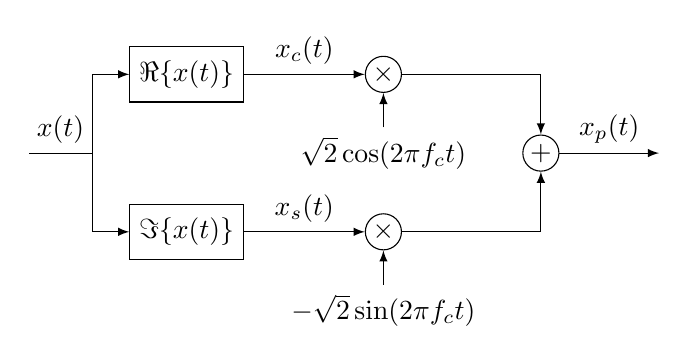
\begin{tikzpicture}[auto, node distance=1.5cm, >=latex]
        % Stili
        \tikzstyle{block} = [draw, rectangle, minimum height=2em, minimum width=3em]
        \tikzstyle{sum} = [draw, circle, inner sep=1pt]
        \tikzstyle{mult} = [draw, circle, inner sep=1pt]
        \tikzstyle{input} = [coordinate]
        \tikzstyle{output} = [coordinate]

        % Nodi
        \node [input] (input) {};
        \node [block, right of=input, node distance=2cm, yshift=1cm] (real) {$\Re\{x(t)\}$};
        \node [block, right of=input, node distance=2cm, yshift=-1cm] (imag) {$\Im\{x(t)\}$};
        
        \node [mult, right of=real, node distance=2.5cm] (mult1) {$\times$};
        \node [mult, right of=imag, node distance=2.5cm] (mult2) {$\times$};
        
        \node [sum, right of=mult1, node distance=2cm, yshift=-1cm] (sum) {$+$};
        \node [output, right of=sum, node distance=1.5cm] (out) {};

        % Oscillatori
        \node [below of=mult1, node distance=1cm] (osc1) {$\sqrt{2}\cos(2\pi f_c t)$};
        \node [below of=mult2, node distance=1cm] (osc2) {$-\sqrt{2}\sin(2\pi f_c t)$};

        % Collegamenti
        \draw [->] (input) -- node {$x(t)$} (0.8,0) |- (real);
        \draw [->] (0.8,0) |- (imag);
        
        \draw [->] (real) -- node {$x_c(t)$} (mult1);
        \draw [->] (imag) -- node {$x_s(t)$} (mult2);
        
        \draw [->] (osc1) -- (mult1);
        \draw [->] (osc2) -- (mult2);
        
        \draw [->] (mult1) -| (sum);
        \draw [->] (mult2) -| (sum);
        
        \draw [->] (sum) -- node {$x_p(t)$} (out);
        
    \end{tikzpicture}
    \caption{Conversion of a baseband signal to a passband signal.}
\end{figure}

\clearpage % --- INIZIO SECONDA COLONNA ---

\textbf{Downconversion} is a bit more involved. Let's say $y_p(t)$ is the signal at the receiver. First of all, the signal is bandpass-filtered in order to have it reject transmission on other frequency bands. Being bandpass, $y_p(t)$ will have a baseband equivalent $y(t) = y_c(t) + j y_s(t)$ such that, just like what we said about the sent signal, we'll have
\begin{equation}
y_p(t) = \sqrt{2} [ y_c(t) \cos(2\pi f_c t) - y_s(t) \sin(2\pi f_c t) ] \;. \tag{2.6}
\end{equation}

% Riquadro Verde
\begin{tcolorbox}[sharp corners, boxrule=0pt, leftrule=2pt, colframe=green!60!black, colback=green!5, left=5pt, top=3pt, bottom=3pt]
    There are ways to extrapolate $y_c(t)$ and $y_s(t)$ using pertinent low pass filters, which need to be realized while knowing the \textbf{carrier frequency} $f_c$:
    \textcolor{green!60!black}{08.2\_pp\_57\_138\_A\_signal\_processing\_perspective, p.63.}
    
    $f_c$ is generally not known precisely; estimating it is a matter tackled by "carrier frequency estimation".
\end{tcolorbox}

The conversion to the baseband is mostly important since most of the processing is done on low frequency signals.

Wireless communications systems send and receive passband signals; those signals are not directly created in passband, though.

\begin{tcolorbox}[frame hidden, sharp corners, boxrule=0pt, leftrule=2pt, colframe=green!60!black, colback=green!5, left=5pt, top=3pt, bottom=3pt]
    Bluetooth is at 5.4GHz; we don't have circuits at those frequencies, as they'd be super intense.
\end{tcolorbox}

What we generally do is to take signals in baseband and then we scale them.

\subsection{Random digression on why radio doesn't transmit on baseband and on ADSL}

\begin{tcolorbox}[frame hidden, sharp corners, boxrule=0pt, leftrule=2pt, colframe=green!60!black, colback=green!5, left=5pt, top=3pt, bottom=3pt]
    Why are radio signals not transmitted in baseband?
    ADSL transmits in baseband to avoid attenuation.
\end{tcolorbox}

Why aren't radio signals transmitted as baseband? We need to go to \textbf{high frequencies if we don't want to make gigantic antennas}.

We studied radio; but what about ADSL? We'd have a twisted pair of cables coming to our house.
Let's say we have a phone. On a cable we're sending voice, on another we're receiving voice; we do so by changing a certain voltage:

\begin{center}
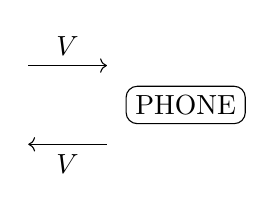
\begin{tikzpicture}
    \node[draw, rectangle, rounded corners] (phone) at (2,0) {PHONE};
    \draw[->] (0, 0.5) -- node[above] {$V$} (1, 0.5);
    \draw[<-] (0, -0.5) -- node[below] {$V$} (1, -0.5);
\end{tikzpicture}
\end{center}

How is it that with just two cables we don't hear a distorted signal (i.e.: how is it that we don't hear our own voice)? We only have one voltage difference!
We could implement FDMA, but it would be impractical! In order to synthesize a frequency, we'd need a crystal and a VCO (voltage controlled oscillator).
What we actually do is use the \textit{forchetta telefonica} (telephone hybrid); we have a circulator which is able to distinguish the incoming and outgoing signal: it cancels the outgoing voltage from the total, getting the incoming voltage as a result.
The telephone hybrid allows us to go from 2 to 4 wires.

\clearpage % --- INIZIO TERZA COLONNA ---

With ADSL we have something like FDMA; we have frequencies up to 4KHz and such (this generally applies to voices; instruments and such will have higher frequencies but we don't really care lol).

\subsection{Random digression on FDD (Frequency Division Duplex) and TDD (Time Divison Duplex)}

FDD and TDD.
When we're transmitting with a radio in SISO, we have an antenna transmitting and an antenna receiving.
When we're transmitting, we can imagine we have a switch which selects the transmitter; when we want to receive, we'll want to select the receiver:

\begin{figure}[h!]
    \centering
    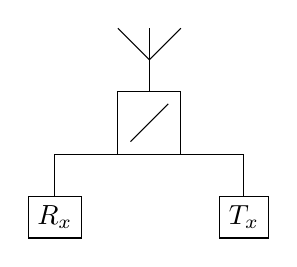
\begin{tikzpicture}[>=latex, scale=0.8]
        % Antenna
        \draw (0,1) -- (0,0.5);
        \draw (0,1) -- (-0.5, 1.5);
        \draw (0,1) -- (0.5, 1.5);
        \draw (0,1) -- (0, 1.5);
        
        % Switch Box
        \draw (-0.5, -0.5) rectangle (0.5, 0.5);
        \draw (-0.3, -0.3) -- (0.3, 0.3); % Switch symbol
        \draw (0, 0.5) -- (0, 0.5); % Connection to antenna

        % Rx Tx
        \node[draw, rectangle] (Rx) at (-1.5, -1.5) {$R_x$};
        \node[draw, rectangle] (Tx) at (1.5, -1.5) {$T_x$};
        
        \draw (Rx) |- (-0.2, -0.5);
        \draw (Tx) |- (0.2, -0.5);
    \end{tikzpicture}
\end{figure}

We also need to be careful about not having contact between receiver and transmitter, as we'd destroy the receiver (which is designed in order to use much smaller voltages)!

\textbf{FDD: Frequency Division Duplex}; we transmit at the same time using different frequencies.
\textbf{TDD: Time Division Duplex}; we have different time slots for transmitting and receiving.

\begin{figure}[h!]
    \centering
    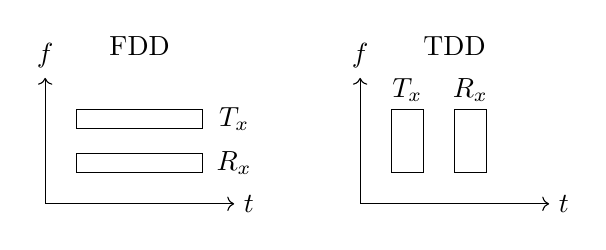
\begin{tikzpicture}[scale=0.8]
        % FDD Graph
        \begin{scope}[xshift=0cm]
            \node at (1.5, 2.5) {FDD};
            \draw[->] (0,0) -- (3,0) node[right] {$t$};
            \draw[->] (0,0) -- (0,2) node[above] {$f$};
            
            \draw[fill=white] (0.5, 1.2) rectangle (2.5, 1.5); \node at (3, 1.35) {$T_x$};
            \draw[fill=white] (0.5, 0.5) rectangle (2.5, 0.8); \node at (3, 0.65) {$R_x$};
        \end{scope}

        % TDD Graph
        \begin{scope}[xshift=5cm]
            \node at (1.5, 2.5) {TDD};
            \draw[->] (0,0) -- (3,0) node[right] {$t$};
            \draw[->] (0,0) -- (0,2) node[above] {$f$};
            
            \draw[fill=white] (0.5, 0.5) rectangle (1, 1.5); \node at (0.75, 1.8) {$T_x$};
            \draw[fill=white] (1.5, 0.5) rectangle (2, 1.5); \node at (1.75, 1.8) {$R_x$};
        \end{scope}
    \end{tikzpicture}
\end{figure}

The problem is that the received signal is much smaller than the transmitted; it's difficult to distinguish them.

Full duplex is now being researched: with full duplex, we use the same frequencies and we transmit in the same time slot.

\section{Complex baseband channel response}The channel for wireless transmission can be modeled as a LTI channel.

If we have a description of the response of the channel to a passband signal, we denote it as
$$
c_p(\tau) \;,
$$
such that we'll have
$$
y_p(t) = (c_p * x_p)(t)
$$
we want to find another \textbf{baseband representation of the channel response}, $c_b(\tau)$, such that
$$
y(t) = [c_b * x](t) \;.
$$

% Riquadro Verde (Time invariance)
\begin{tcolorbox}[sharp corners, boxrule=0pt, leftrule=2pt, colframe=green!60!black, colback=green!5, left=5pt, top=3pt, bottom=3pt]
    About the time invariance: it's more generic to say that the channel is roughly constant over certain intervals of time and frequency.
\end{tcolorbox}

We thus need to find an expression of $c_b$ starting from $c_p$.
Let's look at the various operations we want our baseband channel to implement:

\begin{figure}
    \centering
    
\includegraphics[width=0.7\textwidth]{pictures/image.png}
    \caption{Operations to obtain the baseband channel response from the passband channel response.}
\end{figure}

Let's cover each step:
\begin{enumerate}
    \item We have our channel response, which in the frequency domain might have extra elements on top of the part which interests us (a section of bandwidth $B$ around the frequency $f_c$).
    \item We select only the part of the response which interests us, by multiplying the values for negative and positive frequencies around $f_c$ with two ideal rect functions
    $$
    G_{p, B}(f) = \text{rect}\left(\frac{f-f_c}{B}\right) + \text{rect}\left(\frac{f+f_c}{B}\right) \;,
    $$
    \clearpage % --- INIZIO SECONDA PAGINA ---
    which in the time domain will be
    $$
    g_{p, B}(t) = \underbrace{B \text{sinc}(Bt)}_{\text{env}} \underbrace{2 \cos(2\pi f_c t)}_{\text{shift}}
    $$
    and will be convolved with $c_p(t)$:
    $$
    (c_p(\cdot) * g_{p, B}(\cdot))(t) \;.
    $$
    \item We shift the selected values towards the left, centering around 0 the part of the response which was around $f_c$; this is equal to convoluting with $\delta(f+f_c)$ or, in the time domain, multiplying by the corresponding oscillating signal:
    $$
    e^{-j2\pi f_c t} (c_p(\cdot) * g_{p, B}(\cdot))(t) \;.
    $$
    \item We only select the central component by multiplying our response with an ideal rect centered around 0:
    $$
    G_{b, B/2}(f) = \text{rect}(f/B) \;,
    $$
    which in the time domain will be
    \begin{equation}
    g_{b, B/2}(t) = B \text{sinc}(Bt) \tag{2.12}
    \end{equation}
    and will be convoluted with the result of the previous point:
    $$
    c_b(t) = \left[ \left( e^{-j2\pi f_c (\cdot)} (c_p * g_{p, B})(\cdot) \right) * g_{b, B/2} \right](t) \;.
    $$
\end{enumerate}

% Riquadro Blu: Baseband channel response
\begin{tcolorbox}[colframe=cyan!80!blue, colback=white, boxrule=1pt, arc=2pt]
    \textcolor{cyan!80!blue}{\textbf{Baseband channel response}}

    Since our signal $x(t)$ will be bandlimited, we can actually skip point 2 and get away with an equation such as
    $$
    c_b(t) = [ g_{B/2}(\cdot) * (c_p(\cdot) e^{-j2\pi f_c (\cdot)}) ] (t) \;.
    $$
    \begin{tcolorbox}[sharp corners, boxrule=0pt, leftrule=2pt, colframe=green!60!black, colback=green!5, left=5pt, top=3pt, bottom=3pt]
    In the equation we have a frequency dependent phase shift: we'll see that this is very nasty.
    \end{tcolorbox}
\end{tcolorbox}

% Riquadro Blu: Pseudo-baseband channel response
\begin{tcolorbox}[colframe=cyan!80!blue, colback=white, boxrule=1pt, arc=2pt]
    \textcolor{cyan!80!blue}{\textbf{Pseudo-baseband channel response}}

    We then have that
    $$
    c(t) = c_p(t)e^{-j2\pi f_c t}
    $$
    is the pseudo-baseband channel response, such that if $x(t)$ is bandlimited we can obtain
    $$
    y(t) = [x(\cdot) * c(\cdot)](t)
    $$
    and also such that
    $$
    c_b(\tau) = [g_{B/2}(\cdot) * c(\cdot)](\tau) \;.
    $$
    \begin{tcolorbox}[sharp corners, boxrule=0pt, leftrule=2pt, colframe=green!60!black, colback=green!5, left=5pt, top=3pt, bottom=3pt]
    This comes from my reasoning after \textcolor{green!60!black}{these statements}
    \end{tcolorbox}
\end{tcolorbox}

\clearpage % --- INIZIO TERZA PAGINA ---

The figure shows filtering with passband signals:

\begin{figure}[h]
    \centering
    
\includegraphics[width=0.5\textwidth]{pictures/image copy.png}
    \caption{This image helps understanding why we simplify the equation of the channel
response}
\end{figure}

\section{Q paths complex baseband equivalent}

Let's look at an example in which we have an antenna and a phone; we'll experience different delays $\tau_q$ and different gains $A_q$ for each path followed by the signal:

\begin{figure}[h!]
    \centering
    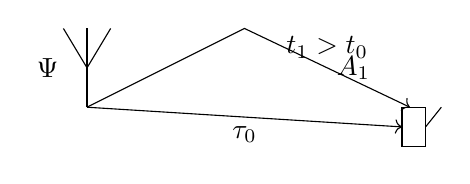
\begin{tikzpicture}[scale=1]
        % Antenna (Tx)
        \node (Tx) at (0,2) {};
        \draw (0,2) -- (0,1.5);
        \draw (0,2) -- (-0.3, 2.5);
        \draw (0,2) -- (0.3, 2.5);
        \draw (0,2) -- (0, 2.5);
        \node at (-0.5, 2) {$\Psi$};

        % Phone (Rx)
        \node (Rx) at (4,1) {};
        \draw (4,1) rectangle (4.3, 1.5); % Phone shape
        \draw (4.3, 1.25) -- (4.5, 1.5); % Small antenna

        % Paths
        % Path 0 (Direct-ish)
        \draw[->] (0, 1.5) -- node[below] {$\tau_0$} (4, 1.25);
        
        % Path 1 (Reflected)
        \draw[->] (0, 1.5) -- (2, 2.5) -- node[above] {$t_1 > t_0$} node[right] {$A_1$} (4.1, 1.5);
        
    \end{tikzpicture}
\end{figure}

We can model such a channel as
\begin{equation}
c_p(\tau) = \sum_{q=0}^{Q-1} A_q \delta(\tau - \tau_q) \;. \tag{2.20}
\end{equation}
The baseband equivalent (according to \textcolor{green!60!black}{"040299"}) will be
\begin{equation}
c_b(\tau) = g_{B/2}(\tau) * \sum_{q=0}^{Q-1} A_q \delta(\tau - \tau_q) e^{-j2\pi f_c \tau_q} \;. \tag{2.21}
\end{equation}

which will give an output
\begin{align}
y(t) &= [c_b * x](t) \nonumber \\
&= \int_{-\infty}^{\infty} \left( g_{B/2}(\tau) * \sum_{q=0}^{Q-1} A_q \delta(\tau - \tau_q) e^{-j2\pi f_c \tau_q} \right) x(t-\tau) \, d\tau \tag{2.22} \\
&= \int_{-\infty}^{\infty} \left( \sum_{q=0}^{Q-1} A_q \delta(\tau - \tau_q) e^{-j2\pi f_c \tau_q} \right) x(t-\tau) \, d\tau \tag{2.23} \\
&= [c * x](\tau) \tag{2.24}
\end{align}
with $c(\tau)$ being the \textbf{complex pseudo-baseband channel response}, since it's shifted but not bandlimited.
$*$ follows from $x$ being bandlimited.

We can obtain the complex baseband channel response from the complex pseudo-baseband channel response as
\begin{equation}
c_b(\tau) = [g_{B/2} * c](\tau) \;. \tag{2.25}
\end{equation}

\section[Time discretization]{Time discretization: discrete representation of the channel $c[\ell]$ (+critical sampling)}

Since the channels are bandlimited, we can sample with a period $T \le 1/B$ (equality is what we'll call \textit{critical sampling}) and discretize the input and the channel.

Let's say we have $x(t), y(t)$ represented by their discrete-time samples with $T=1/B$; we want to find a channel such that
\begin{equation}
y[n] = \sum_{\ell} c[\ell]x[n-\ell] \;. \tag{2.27}
\end{equation}

% Riquadro Viola: FYI
\begin{tcolorbox}[colframe=violet!60!white, colback=white, boxrule=1pt, arc=2pt]
    \textcolor{violet}{\textbf{FYI}}

    This is a noiseless \textcolor{green!60!black}{frequency selective}, \textcolor{green!60!black}{unitary gain channel model}, as will be shown in (2.80).
\end{tcolorbox}

If we try and discretize the convolution $[c_b * x]$ (with reference to (2.25) and previous equations) with a step $d\tau \to T$, we get
\begin{align}
y(nT) &= (c_b * x)(nT) \nonumber \\
&= \int_{-\infty}^{\infty} c_b(\tau)x(nT - \tau) \, d\tau \tag{2.28} \\
&\approx \sum_{\ell} c_b(\ell T) x(nT - \ell T) T \tag{2.29} \\
&= \sum_{\ell} T c_b(\ell T) x[n-\ell] \;, \tag{2.30}
\end{align}
which, when compared with the equation of $y[n]$ in (2.27), will point us to conclude that $c[\ell] \approx T c_b(\ell T)$.

We can conclude that the discrete time equivalent in (2.27) for any baseband or pseudo-baseband channel is obtained by:

\clearpage % --- INIZIO SECONDA PAGINA ---

\begin{enumerate}
    \item Taking the generic channel response $c(\tau)$
    \item Filtering it with the low-pass filter $T g_{B/2}(\tau)$, thus obtaining $c_b(\tau)$
    \item Sampling it at $\tau = \ell T$
\end{enumerate}

% Riquadro Blu: Discrete time baseband channel equivalent
\begin{tcolorbox}[colframe=cyan!80!blue, colback=white, boxrule=1pt, arc=2pt]
    \textcolor{cyan!80!blue}{\textbf{Discrete time baseband channel equivalent}}

    It will thus be
    $$
    c[\ell] = [T g_{B/2} * c](\tau)|_{\tau = \ell T}
    $$
    or, if the channel is already bandlimited,
    \begin{equation}
    c[\ell] = [T c(\tau)]|_{\tau = \ell T} \;. \tag{2.31}
    \end{equation}
\end{tcolorbox}

% Riquadro Verde (Note)
\begin{tcolorbox}[sharp corners, boxrule=0pt, leftrule=2pt, colframe=green!60!black, colback=green!5, left=5pt, top=3pt, bottom=3pt]
    Where the $T$ is introduced in order to keep the energy constant.
    
    If we want to deal with signal theory, professor suggests to look at "unified signal theory".
\end{tcolorbox}

What's important here is that we'll forget about the continuous time domain and we continue with the discrete time domain:

% Riquadro Giallo (Riferimento)
\begin{tcolorbox}[colframe=yellow!80!orange, colback=white, boxrule=1pt, arc=2pt]
    \textcolor{green!60!black}{\small \ 08.2\_pp\_57\_130\_A\_signal\_processing\_perspective, page 10}

    In light of the connection established between passband signals, bandlimited baseband signals, and discrete-time signals, most results in this book are formulated directly in discrete time. Although actual signals are not exactly bandlimited since they are time-limited, and the filters in the front-ends are never ideal, signals are close to bandlimited as they are mandated to have low adjacent channel interference.
    Commercial systems also feature analog-to-digital and digital-to-analog converters with finite precision. Normally, perfect conversion is assumed in the design stages and then the required tolerances are investigated after the fact via simulation. Quantization and reconstruction errors are not part of the models in this text.
\end{tcolorbox}

\section[Pulse shaping: from digital signal to an analog]{Idea of pulse shaping: from a digital signal $x[n]$ to an analog signal}

Pulse shaping: the book mentions it, but it's not really important.

% Riquadro Giallo (Riferimento)
\begin{tcolorbox}[colframe=yellow!80!orange, colback=white, boxrule=1pt, arc=2pt]
    \textcolor{green!60!black}{\small 08.2\_pp\_57\_130\_A\_signal\_processing\_perspective, page 10}

    The sampling and reconstruction that we have applied to discretize the transmit-receive relationships can be interpreted as basic modulation and demodulation schemes, whereby the complex symbols that make up the codewords are embedded onto $x(t)$ and then extracted from $y(t)$.
\end{tcolorbox}

The basic concept of pulse shaping is to link the symbols of the message we're transmitting, $x[n]$, with the actual continuous time signal, $x(t)$.

\clearpage % --- INIZIO TERZA PAGINA ---

If we know $x[n]$, we might think ab using $\text{sinc}$ for interpolation; problem is that it is not causal!
What we generally do then is to use the \textbf{square root raised cosine}.

No matter what functions we'll use for interpolation at the transmitter, we'll call it $g_{tx}$.
At the receiver we'll use a different function, $g_{rx}$, to filter what we received.

We can generally \textbf{reconstruct the signal through interpolation as}
\begin{equation}
x(t) = \sum_{n} x[n] g_{tx}(t - nT) \;, \tag{2.41}
\end{equation}
where $g_{tx}(\cdot)$ is the transmit pulse shape.

At the receiver, we'll then use a specific filter which in reality cannot be the ideal low-pass filter $g_{B/2}(\cdot)$ described in (2.18): it will be a modified filter $g_{rx}(-)$.

The \textbf{composite pulse shape} is thus defined by combining the two pulse shapes, as
\begin{equation}
g(\tau) = [g_{tx} * g_{rx}](\tau) \;. \tag{2.42}
\end{equation}

% Riquadro Grigio: Skipped
\begin{tcolorbox}[colframe=gray, colback=white, boxrule=1pt, arc=2pt]
    \textcolor{gray}{\textbf{Skipped}}

    Possible definitions of $g(\tau)$ can be found from \textcolor{green!60!black}{08.2\_pp\_57\_130\_A\_signal\_processing\_perspective, page 13} to \textcolor{green!60!black}{08.2\_pp\_57\_130\_A\_signal\_processing\_perspective, page 15}. Professor completely skipped them.

    \hfill \textcolor{red}{\Large Week 17 Nov - 23 Nov} % O semplicemente textcolor{red}{Week 17 Nov...} se non hai font speciali
\end{tcolorbox}

\section[Channel models]{Channel models (frequency selective, FIR, flat channel); channel normalization and average symbol energy; vector representation of a SISO FIR channel}

An important thing is the normalization of the channel; people normally make lots of mistakes about this.

We have the model defined in (2.19).
We can model such a channel as
\begin{equation}
c_p(\tau) = \sum_{q=0}^{Q-1} A_q \delta(\tau - \tau_q) \;. \tag{2.19}
\end{equation}

If we don't pay attention, this channel could be amplified. We need to pay attention because the energy of the channel is
$$
\sum |A_q|^2 \;,
$$
which might be greater than 1.

% Riquadro Verde
\begin{tcolorbox}[sharp corners, boxrule=0pt, leftrule=2pt, colframe=green!60!black, colback=green!5, left=5pt, top=3pt, bottom=3pt]
    What's important is the ratio between the noise and the amplification of the channel (which comes from the antenna itself, its directionality etc etc): the gain is in respect to an isotropic antenna.
\end{tcolorbox}

\end{document}